%% LyX 2.1.3 created this file.  For more info, see http://www.lyx.org/.
%% Do not edit unless you really know what you are doing.
\documentclass[english]{article}
\usepackage[T1]{fontenc}
\usepackage[latin9]{inputenc}
\usepackage{geometry}
\geometry{verbose,tmargin=2.8cm,bmargin=2.8cm,lmargin=2.6cm,rmargin=2.6cm}
\usepackage{textcomp}
\usepackage{graphicx}

\makeatletter

%%%%%%%%%%%%%%%%%%%%%%%%%%%%%% LyX specific LaTeX commands.
%% Because html converters don't know tabularnewline
\providecommand{\tabularnewline}{\\}

\makeatother

\usepackage{babel}
\begin{document}

\title{DAAD Short-term grant Application}

\maketitle

\section*{Applicant: Lic. Kevin Speyer}


\section{Previous Research Work}

The candidate, Kevin Speyer, holds years of experience performing
research in polymer physics and Soft Matter by computer simulations.
He published two papers in international peer-reviewed journals. His
main working subjects are Polymer Brushes, composed of semiflexible
chains anchored to the walls of a nano-channel, and the interactions
between this soft substrate and liquid flow in nano-fluidic systems.
A wide range of physical quantities are measured in these systems,
from the molecular degrees of freedom to thermodynamic or rheological
properties. The work is performed by means of Molecular Dynamics simulations,
in the context of Statistical Mechanics theory. The applicant hold
PhD CONICET scholarship working in the Theory and Simulation of Soft
Matter Group of the National Atomic Energy Commission (CAC-CNEA) in
Argentina. The group has a history of collaboration with the Soft
Matter Theory Group of Prof. Dr. Marcus M�ller in G�ttingen. The applicant's
supervisor, Dr. Claudio Pastorino, has a vast experience in polymer
physics theory and simulation, and is now a researcher in CNEA and
CONICET at CAC-CNEA

In his Diploma Thesis (MS equivalent), entitled ``Simulation of simple
liquids confined in soft channels'', the candidate studied a nanochannel
with confining surfaces coated with grafted polymers. In this work,
the interaction between the liquid and the grafted polymers was analyzed
in equilibrium and in flow conditions. This first study was focused
on the influence of the bending rigidity of the semiflexible polymers
on the static and dynamical properties of the system. The interaction
between the soft substrate and the liquid is hydrophobic, giving rise
to a Cassie\textendash Baxter state. Equilibrium properties such as
brush height and bending energy were measured, varying the grafting
density (number of chains per surface area) and the stiffness of the
polymers. The characteristics of the brush\textendash liquid interface
and the morphology of the polymer chains supporting the liquid were
studied for different bending rigidities. Non-equilibrium simulations
were performed, moving the walls of the channel in opposite directions
at constant speed, obtaining a Couette velocity profile in the bulk
liquid. The molecular degrees of freedom of the polymers are studied
as a function of the shear rate. The violation of the no-slip boundary
condition and the slip properties were analyzed as a function of the
shear rate, grafting density and bending stiffness. At high grafting
densities, a finite slip length independent of the shear rate or bending
constant was found, while at low grafting densities a very interesting
non-monotonic dependence on the bending constant is observed. This
work was published in the journal \textit{Soft Matter}\cite{Speyer_15}.

In another study, the candidate analyzed a system composed of a liquid
droplet in a nanochannel, coated with semiflexible hydrophobic polymers
by means of non-equilibrium molecular dynamics simulations. The studied
system is then a moving droplet in a slit-like channel, coexisting
with its vapor phase. The polymer chains, grafted by the terminal
bead to the confining walls, are described by a coarse-grained model
that accounts for chain connectivity, excluded volume interactions
and local chain stiffness. The rheological, frictional and dynamical
properties of the brush are explored over a wide range of persistence
lengths. A rich behavior of polymer conformations and concomitant
changes in the friction properties are found over the wide range of
studied polymer stiffnesses. A rapid decrease in the droplet velocity
was observed as the rigidity of the chains is increased for polymers
whose persistence length is smaller than their contour length. A strong
relation between the internal dynamics of the brush and the droplet
transport properties is found, which could be used to tailor flow
properties by surface functionalization. The monomers of the brush
layer, under the droplet, present a collective \textquotedblleft treadmill
belt\textquotedblright{} like dynamics which can only be present due
the existence of grafted chains. The changes in spatial extension
upon variations of polymer stiffness are described, with bidimensional
velocity and density profiles. The deformation of the polymer brushes
due to the presence of the droplet is analyzed in detail. Lastly,
the droplet\textminus gas interaction is studied by varying the liquid
to gas ratio, observing a speed increase for droplets that flow close
to each other, compared to a train of droplets that present a large
gap between consecutive droplets. These results were recently published
in \textit{Langmuir\cite{doi:10.1021/acs.langmuir.7b02640} }\textit{\emph{journal}}\textit{.}

The candidate works on a daily basis on large computation clusters,
running coarse grain simulations in compiled languages, and performing
post-processing statistical analysis with scripting languages (python,
awk). He is familiar with various visualization tools for 3D atom
dynamics (Visual Molecular Dynamics), color plots and data visualization
(python, Xmgrace, gnuplot). He has experience in High Performance
Computing, parallelizing code in non-trivial processes.


\section{Working Project}

\noindent Using large-scale computer simulation of coarse-grained
polymer models we propose the study of non-equilibrium behavior of
active polymer brushes. This soft-matter system mimics active biological
systems capable of directed transport. The system also exhibits an
intricate, non-equilibrium single-chain dynamics (``tumbling motion''),
and our simulation study will elucidate to what extent the individual
molecular motions are coupled and synchronized (spatiotemporal correlations)
and how the molecular motion interacts and dictates the collective
structure and flow field. The project takes advantage also of the
strong experience of the applicant in semi-flexible polymer brushes,
by adding the important element of chain activeness. A given energy
per unit time will be injected in each grafted polymer to obtain a
self-sustained oscillation of the polymers, which will give raise
to a collective behavior depending on chain-stifness, grafting density
and the properties of the liquid. The student will have the opportunity
to learn about modern concepts of non-equilibrium statistical mechanics
and state-of-the-art simulation techniques on clusters of CPUs and
GPUs.

\vspace*{0.5cm}



\subsection{\noindent Goals}

Polymers in flow have attracted abiding interest by experimental and
theoretical researchers. By irreversibly grafting a polymer onto a
solid substrate one fabricates brush coatings that are both, mechanically
stable as well as versatile for tuning the wettability and friction
of the coated surface.\cite{Zhao00} In our previous collaboration
we have developed and utilized coarse-grained computer simulations
to study polymer brushes under flow,\cite{Pastorino_06,Pastorino_07,Pastorino_09,Mueller_09}
studied how the brush coating dictates the hydrodynamic boundary condition,\cite{Mueller_08,Leonforte_11}
and studied the tumbling motion of the individual grafted macromolecules
and the concomitant reversal of the near-surface flow under shear.\cite{Mueller_08b,Pastorino_14}.
We propose now to extend our study to collective phenomena in active
polymer brushes, which exhibit collective, non-equilibrium phenomena.


\vspace*{0.3cm}


\noindent The coating of the surfaces with tethered polymers alters
the flow properties in the ultimate vicinity of the coated surface.
These boundary effects become particular important in microfluidic
devices that manipulate confined liquids at the pico-liter scale,
electroosmotic flow, or vascular biological systems.\cite{Weinbaum_03}
Much interest has focused on driving the liquid motion externally,
e.g., by a pressure difference, shear of confining boundaries, or
an electric field. Such conditions are particularly relevant for applications
such as lab-on-chip devices,\cite{Squires_05,tabelling_microfluidics}
controlled drug delivery, functionalized surfaces and sensing at the
nano-scale.

Active particles and polymers in biological context or active, synthetic
realizations constitute an alternative driving mechanism that has
attracted much attention recently. In these systems, the active entities
possess internal degrees of freedom that enable them to take energy
from the environment and perform mechanical work in the form of, e.g.,
systematic movements. Active systems under study range from bacteria\cite{Ramaswamy_10}
or spermatozoa, to smaller functional units of cells and micro-organisms
such as cilia, flagella and molecular motors.\cite{Cates_11,Elgeti_15}
These last cases include also so-called micro-swimmers of biological
origin, such as opalinas and chlamydomonas or synthetic experimental
systems such as self-propelled droplets, catalytic Janus colloids
or thermophoretic nano-particles.\cite{Elgeti_15} Understanding the
mechanisms how the coupling among active units results in directional
motion \cite{Elgeti_13,Lauga_09,Bennett_2013,Backholm_14,Pande_15}
and the collective states of these active materials is of great current
interest.

The coordinated motion of cilia, which are comprised of active, semiflexible
filaments anchored to a surface, can give rise to directed motion
of micro-organisms in nature or to pumping of fluids in certain tissues.
For example, cilia in the human respiratory tract pump viscous fluids
away from the lungs or propel dust particles out of the body. This
amazing function and the efficiency of cilia transport has stimulated
research groups to design synthetic analogues in order to regulate
flow or particle motion in microfluidic devices.

We propose to study planar nano-channels coated by active polymers,
end-grafted to the confining walls of a narrow slit channel. The system
is a generalization of semi-flexible polymer brushes, which have been
previously studied thoroughly by the applicant. For this project we
add a protocol energy injection which gives raise to self-sustained
movement. Fig. \ref{fig_brushes} presents preliminary examples of
these systems. We have already developed a coarse-grained beating
model for the individual chains that captures the essential features
of the movement of typical active filaments, such as cilia or flagellae.
A cilium filament, for example, presents a power stroke and a recovery
stroke. In the former the cilium stretches out and moves rather fast
in one direction. In the recovery stroke, in turn, the cilium bends
and slowly retracts.\cite{Elgeti_15} We reproduced this asymmetric
beating pattern with our coarse-grained model. This motion results
from an internal activity or is driven by coupling to an external,
time-dependent field. A deep characterization of this model must be
done in dry brushes, to study then the liquid transport due to the
collective motion of active grafted polymers. Specifically, we propose
two types of couplings between self-sustained polymer chains. The
first one is given by the direct interaction between neighboring chains
and the second one is an harmoning coupling of neighboring chains
close to the grafting point. 

\providecommand{\tabularnewline}{\\} 
\begin{figure}
\begin{centering}
\begin{tabular}{ccc}
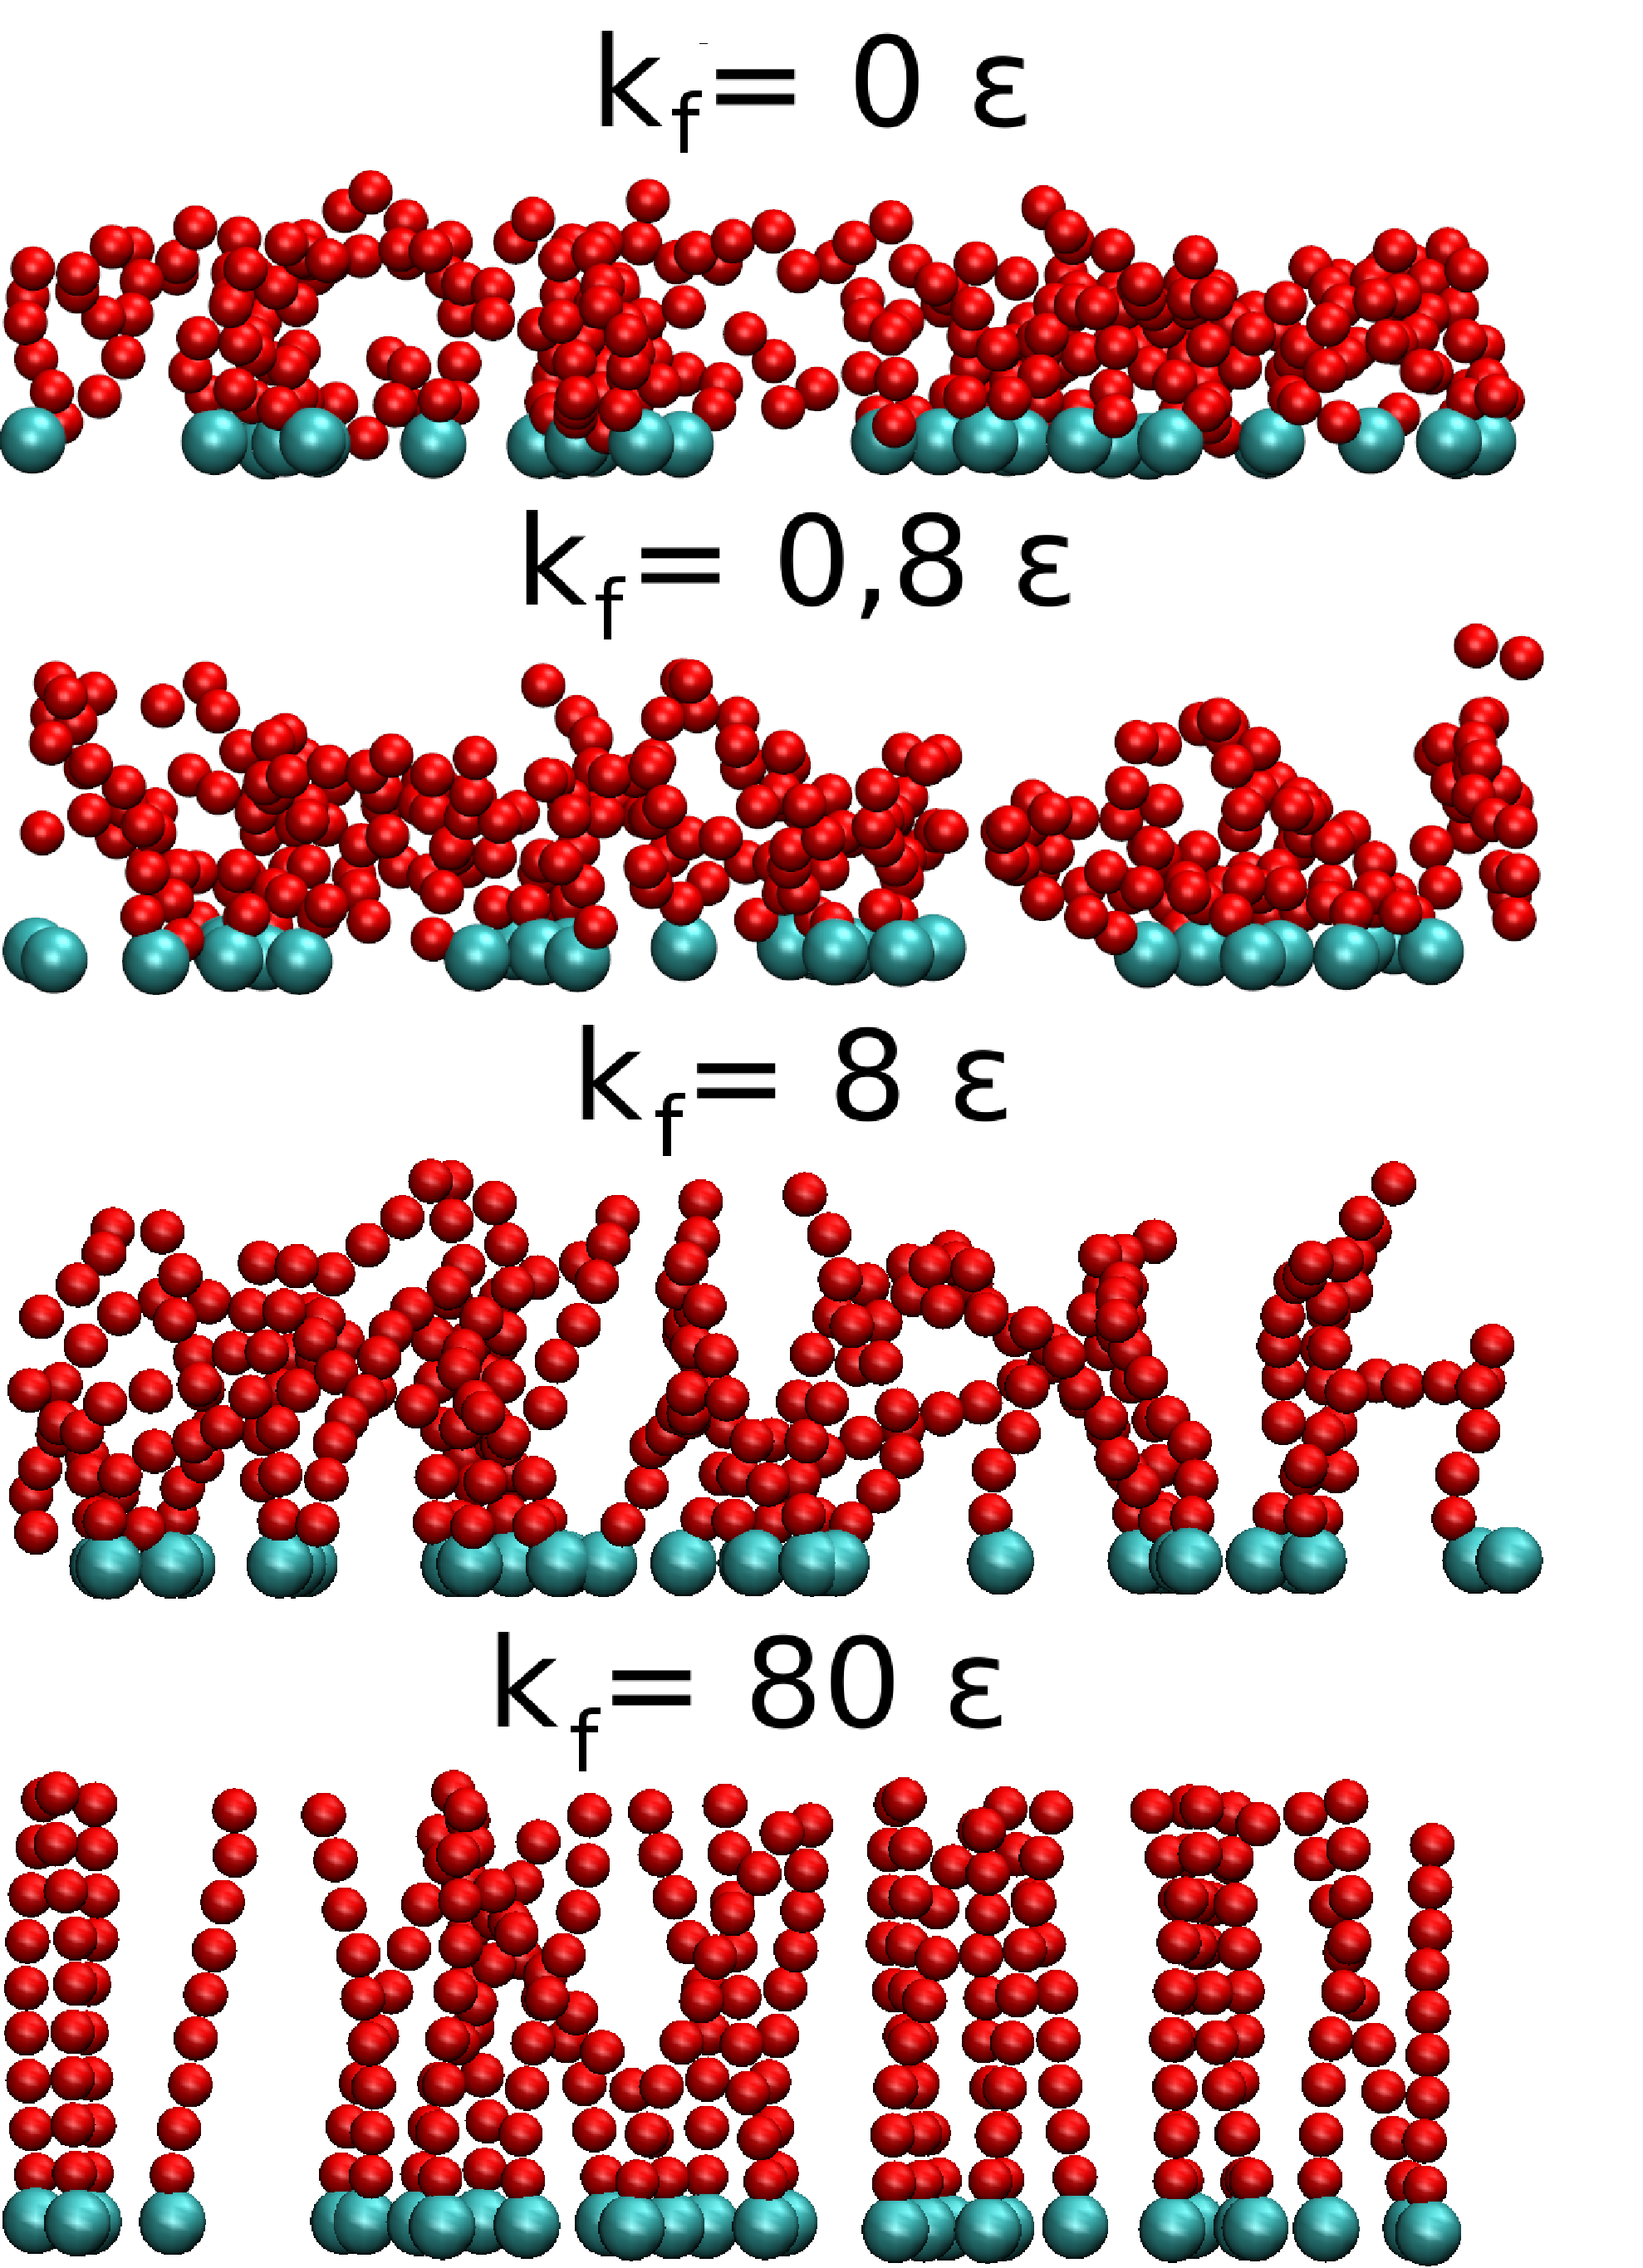
\includegraphics[clip,width=0.26\columnwidth]{figs/Brushes2}  & 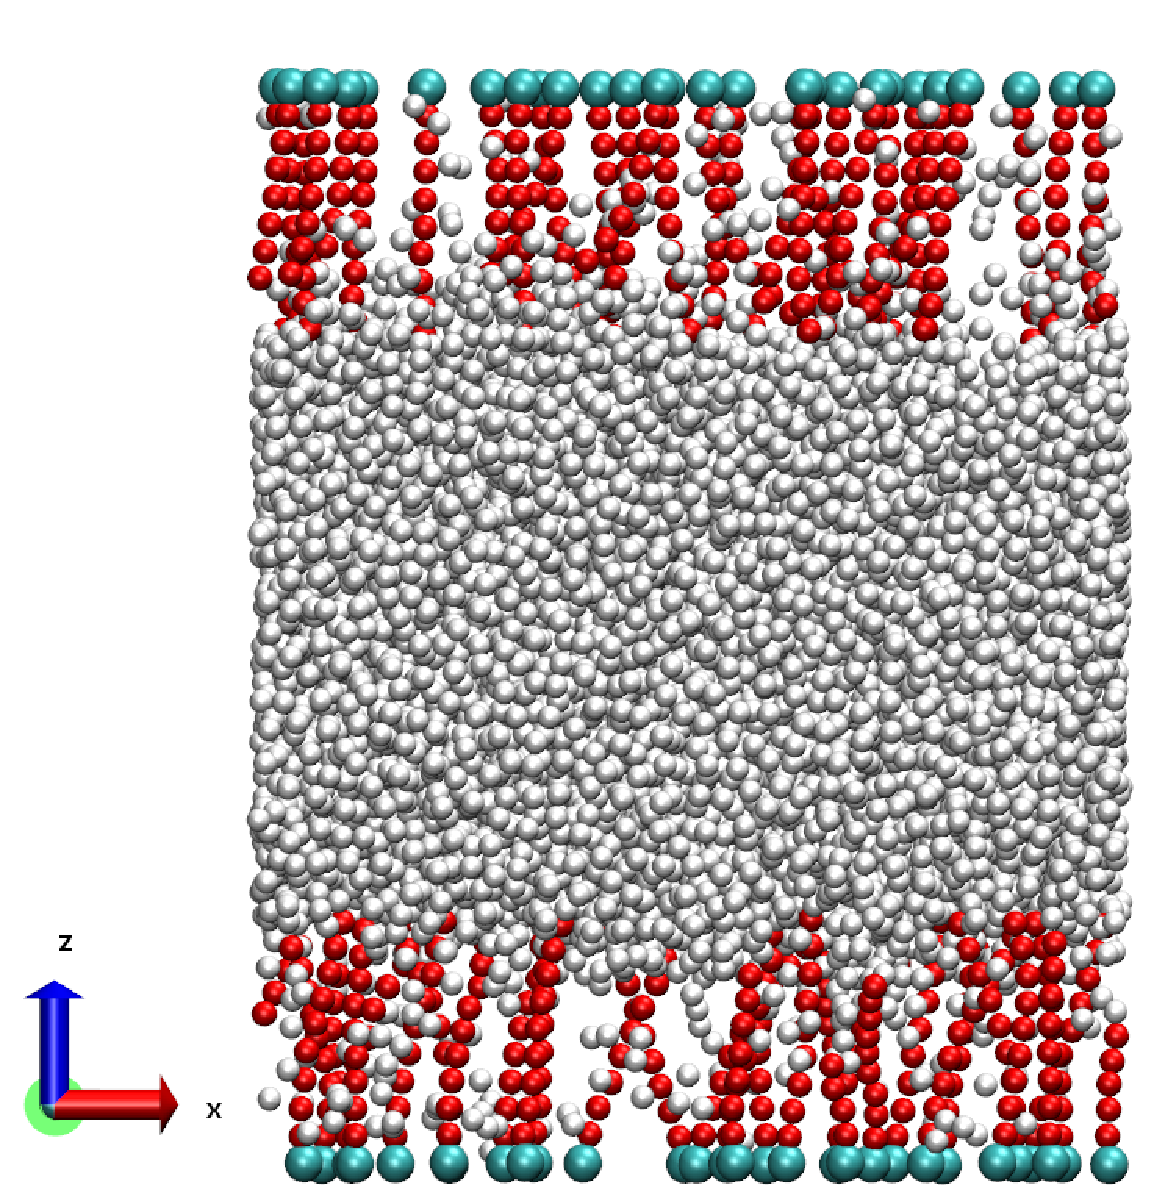
\includegraphics[clip,width=0.28\columnwidth]{figs/Muestra1}  & 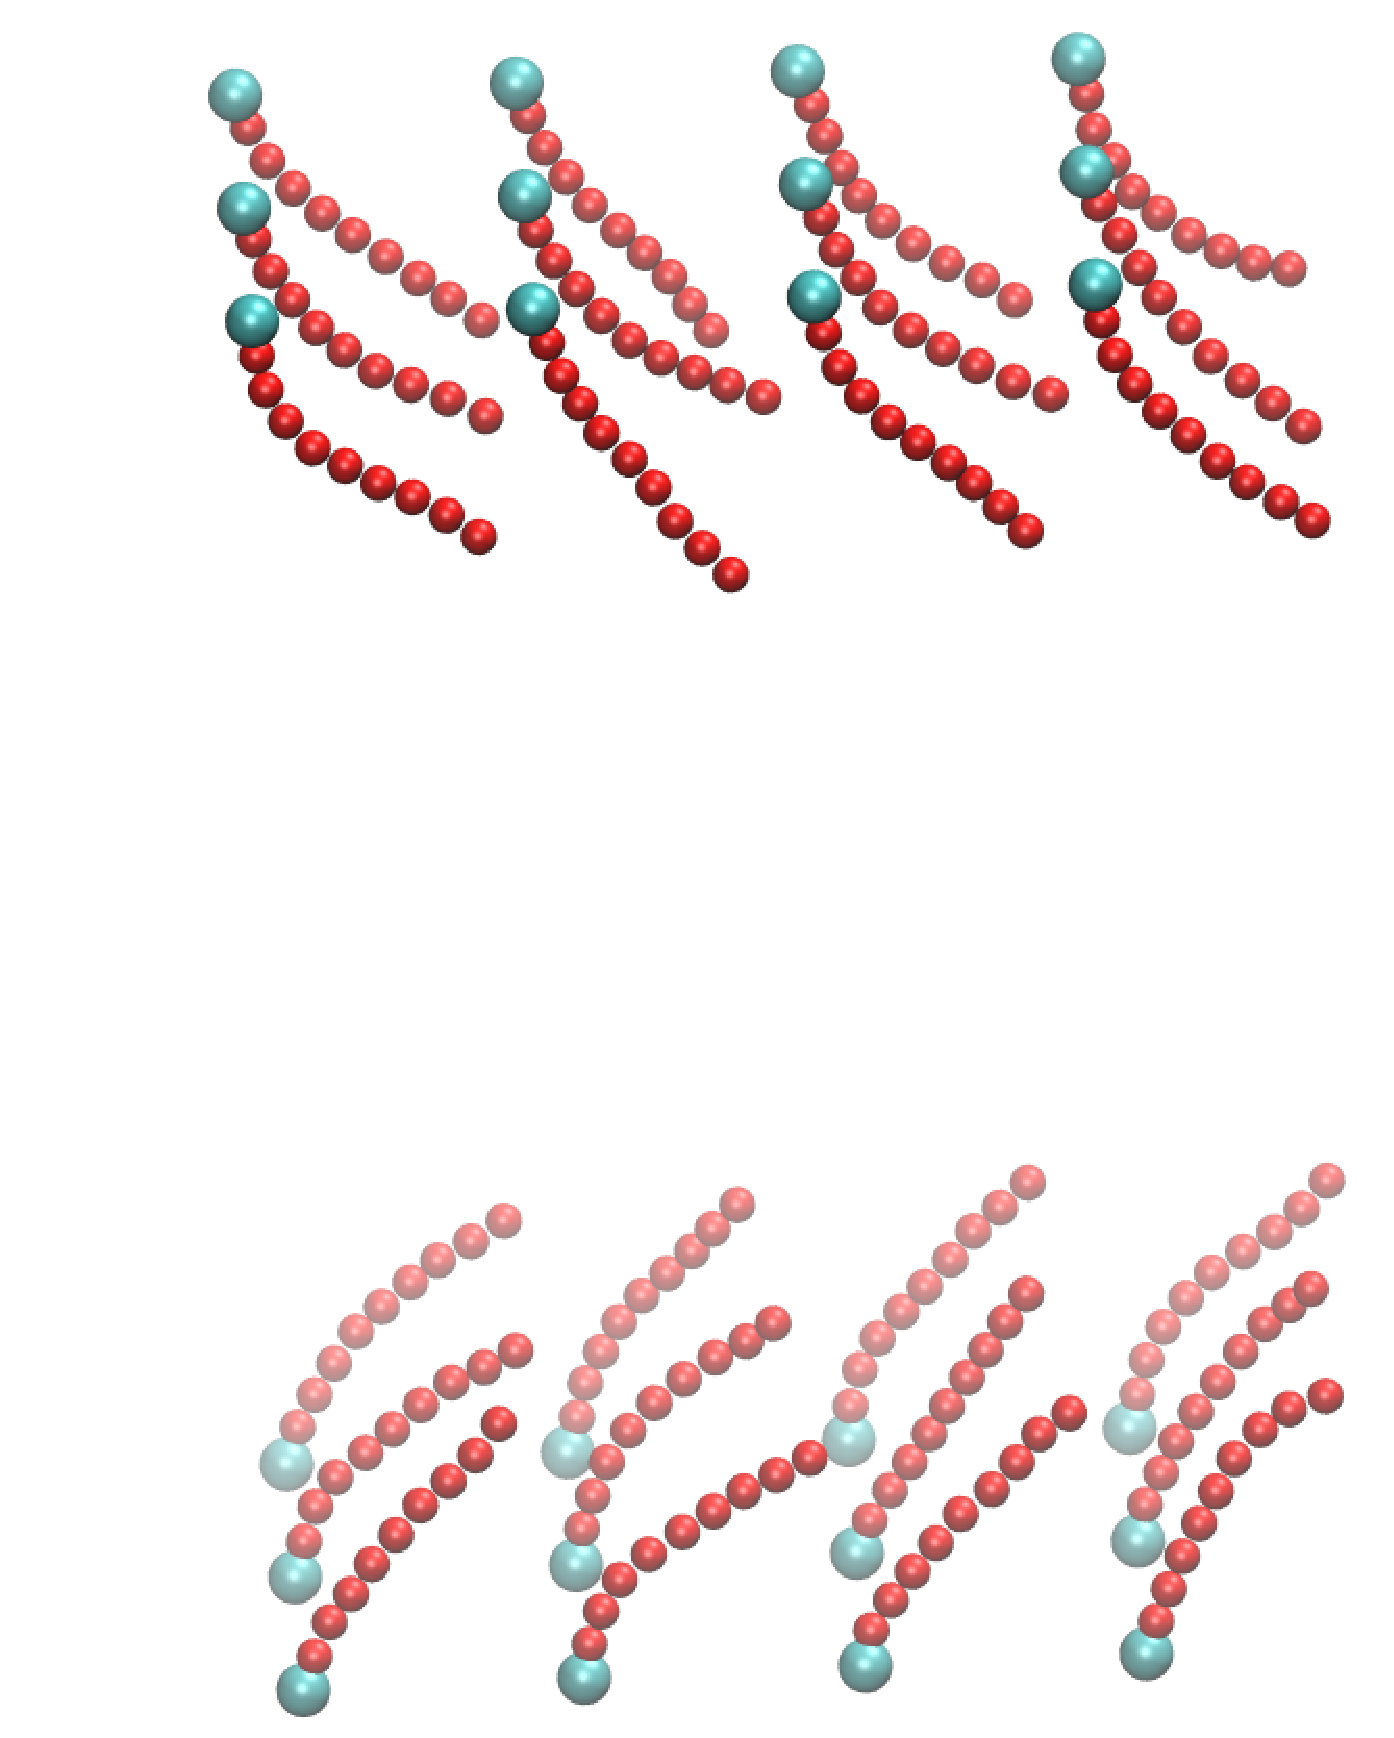
\includegraphics[clip,width=0.28\columnwidth]{figs/active_brush}\tabularnewline
\end{tabular}
\par\end{centering}

\protect\caption{Left panel: Grafted polymer layers with increasing stiffness, which
is parameterized by the bending constant $k_{f}$. Center panel: Planar
channel filled with liquid confined between two stiff polymer brush
layers with $k_{f}=80$. Right panel: Illustration of an active brush
oscillating with the same phase (phase-locked state, grafting points
arranged on square lattice). \label{fig_brushes} }
\end{figure}


The applicant will study the synchronization of the polymers of the
active brush and their interaction with the liquid: 
\begin{itemize}
\item What is the relative importance of mechanical/steric and hydrodynamic
interactions in the collective dynamics of the polymer chains? 
\item How do synchronized, active brushes produce directed flow in a nano-channel? 
\item What are the effects of the interaction with the liquid on the local
dynamics of active chains and synchronization, when the liquid is
exposed to (external) shear? 
\item Methachronal waves are frequently observed in biological cilia, i.e.,
there are regions of perfect synchronization surrounded by disordered
beating patterns. We want to address also the origin of these collective
features and the relationship with the liquid flow in the channel. 
\end{itemize}

\subsection{\noindent Methodology}

We will use coarse-grained molecular dynamics simulations of coarse-grained
bead-spring models. The active polymer brushes are described by the
Kremer-Grest model, \cite{Grest_86,Kremer_90} where segments interact
via a Lennard-Jones potential describing the harsh excluded volume
of individual segments. A Finite Non-linear Extensively Elastic (FENE)
potential accounts for the chain connectivity. We have used this model
in our previous joint work on polymer brushes.\cite{Pastorino_06,Pastorino_09,Pastorino_14}
Additionally, we apply a harmonic bending potential between two consecutive
bonds that connect a given monomer with its two nearest neighbors
in order to tune the rigidity of the semi-flexible polymer chain.\cite{Speyer_15}
The applicant has an important experience in the study of semi-flexible
brushes under flow and has implemented the bending rigidity of the
polymer chains.\cite{Speyer_15,doi:10.1021/acs.langmuir.7b02640}
Importantly the combination of harsh excluded-volume interactions
between segments and a maximal bond length guarantees that chain contours
cannot cross through each other in the course of the simulation. These
entanglement effects that dramatically alter the dynamics in dense
melts of long polymers, may be important for the synchronization of
the active polymers.

We are planning the use of molecular dynamics simulation with a DPD
(or Lowe-Anderson) thermostat.\cite{DPD1,Lowe} This pairwise thermostat
obeys translation invariance and locally conserves momentum, thereby
duly accounting for hydrodynamic interactions that are mediated via
the explicit solvent.\cite{Mueller_09,Pastorino_07,Pastorino_15}
We have experience in using this simulation techniques to study isothermal
flows in nano-channels. \cite{Mueller_08b,Pastorino_15,Pastorino_14,Leonforte_11}

The simulations of active brushes will be performed by a MPI-parallel
simulation code that is well suited for computer clusters, but the
applicant will learn the use and programing of a GPU-program that
is based on the HOOMD code (see http://glotzerlab.engin.umich.edu/hoomd-blue),
in his visit to G�ttingen. %%CP: does not compile refs properly
%%\footnote{\url{http://glotzerlab.engin.umich.edu/hoomd-blue}}
The latter allows for large-scale simulations on clusters of GPUs
that are available at the von-Neumann Institute for Computing in J�lich
and the Argentinian group will strongly benefit of this knowledge.


\subsection{Detailed work plan}
\begin{itemize}
\item Channel with explicit solvent: synchronization and hydrodynamic coupling

\begin{itemize}
\item An explicit solvent will be added to channel coated by active brushes,
described by Lennard-Jones particles, to account for momentum conservation
and the concomitant hydrodynamic interactions, taking advantage of
the experience of the German group. 
\item We will analyze the effect of solvent-mediated hydrodynamic coupling
between active chains and characterize changes in the collective chain
dynamics, as compared to the case of elastic coupling alone (in dry
brushes). 
\end{itemize}
\item Liquid flow with synchronized chain dynamics

\begin{itemize}
\item Imposing coordinated movement to the chains, mimicking typical cilia
dynamics, we will study the flow generated in the solvent. 
\item Upper and lower active brush layers of the slit channel will be studied
as a function of polymer beating frequency, amplitude, and direction.
Directed flow in the vicinity of the individual active brush layers
can be achieved by choosing parameters that result in synchronization
(obtained in the previous task using the ``dry channel''), or by
imposing a phase-locked dynamics with a time-dependent external force. 
\item Special interesting cases are in-phase movement of active upper and
lower brushes and anti-phase movement of upper and lower grafted layers.
If the polymers drive locally the fluid, the in-phase movement is
expected to produce a plug flow, whereas the anti-phase movement results
in shear flow. 
\item A parallelization scheme with GPU of some parts of the code will be
studied and implemented by the applicant wiht the help of the Prof.
M�ller and his group. 
\end{itemize}
\end{itemize}
\bibliographystyle{plain}
\bibliography{biblio,c_refs,bibtex}

\end{document}
